% LaTeX file for resume 
% This file uses the resume document class (res.cls)

%\documentclass[margin]{res} 
\documentclass[margin]{res}
\usepackage{graphicx}
\usepackage{wrapfig}
\graphicspath{ {/Users/haynes/Downloads/} }
%\topmargin=-0.4in
%\oddsidemargin -.25in
%\evensidemargin -.25in
%\textwidth=5.0in
%\textheight =10.4in
%\usepackage[margin=1.0in]{geometry}
\usepackage{multicol}
% the margin option causes section titles to appear to the left of body text 
%\textwidth=5.5in % increase textwidth to get smaller right margin
%\usepackage{helvetica} % uses helvetica postscript font (download helvetica.sty)
%\usepackage{newcent}   % uses new century schoolbook postscript font 
\tolerance=1
\emergencystretch=\maxdimen
\hyphenpenalty=10000
\hbadness=10000
\begin{document} 
 
\name{William Haynes Heaton, M.D.\\ [12pt]} % the \\[12pt] adds a blank line after name
 
%\address{  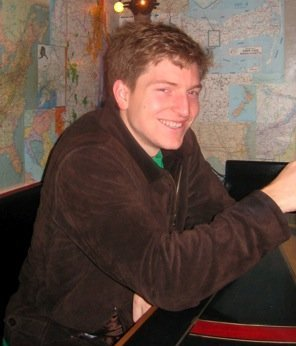
\includegraphics[scale=0.4]{pic} 1552 East Gate Way \#231 \\ Pleasanton CA, 94566 \\
  %      (256) 648-6432 \\ https://github.com/wheaton5 \\
    %    www.haynesheaton.com} 
%\begin{wrapfigure}{l}{0.25\textwidth}
%\centering
%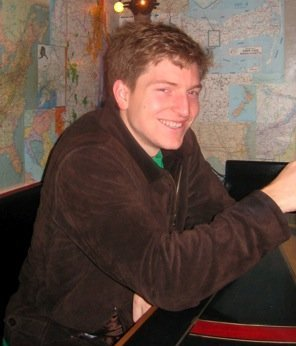
\includegraphics[scale=0.4]{pic}
%\end{wrapfigure}
\address{ Grange Rd. Selwyn College \\ Cambridge, Cambridgeshire, CB3 9DQ \\
        +44 7955 343268 \\ https://github.com/wheaton5 \\
        www.haynesheaton.com}


 
\begin{resume} 
\section{Education} 

PhD (current, expected 2021) \hfill Sanger Institute, University of Cambridge, Cambridge, UK \\
MD May 2011 \hfill Brown Medical School, Providence, RI \\ 
Computer Science/Computational Biology May 2007 \hfill Brown University, Providence, RI 
\section{Industry \\Experience}

{\bf Senior Scientist}, 10X Genomics \hfill 2014-2017 \\
Algorithm and software development on genomics platform bringing long range genetic information to nextgen short-read sequencing. We use a microfluidic system to attach the same barcode to every read originating from a long DNA molecule while different molecules get different barcodes with high probability. This data type is not dissimilar from Moleculo, complete genomics LFR, or illumina CPT seq but since it is droplet based instead of plate based, we are able to have millions of different partitions/barcodes instead of thousands.
\begin{itemize}
\item Developed new linked-read aligner ``Lariat" based on BWA-mem which takes into account the molecule information when finding its mapping. This produces fewer mismapped reads and is able to map into many repeat regions of the genome with high confidence. (lead on this project)
\item Invented novel phasing probabilistic model which is able to filter variants that do not segregate correctly on haplotype lines. 
\item Head of short variant calling and data analysis, metrics, ground truth analysis of short variants.
\item Created a system of haploid variant calling to improve sensitivity. 
\item Worked with biochemists and chemists to create data metrics that allow them to continuously improve the data quality.
\end{itemize}


{\bf Sr Software Engineer: Scientific Computing}, GNS Healthcare, Cambridge MA \hfill 2013 - 2014 \\
Part of a team working on causal bayesian network machine learning with MCMC to sample graph structure of the bayesian nets. \\
\begin{itemize}
\item Contributed to methods in post learning simulation, analysis, and clustering.
\item Developed and supported Amazon EC2 execution of our platform using Starcluster.
\item Created distribution process for our post learning simulation using Hadoop on Amazon Elastic map reduce. 
\end{itemize}


{\bf Computational Scientist,} Nabsys, Providence RI \hfill 2011 - 2013 \\
Developed algorithms for a nano channel DNA mapping startup. Collaborated with Biochemistry and Electrical Engineering teams as well as consulting CS professors to make novel methods addressing data produced by a unique assay -- long (10s-100s of kilobases) DNA fragments with tag molecules attached to sequence specific sites are run through a solid-state nano-detector, creating data analogous to ordered restriction maps (or bionano genomics data). \\

\begin{itemize} %\itemsep -2pt  % reduce space between items
\item Developed genetic distance map de novo assembly software with computational biologist Peter Goldstein. 
\item Created novel multiple alignment using a probabilistic, graph theoretic approach. This allowed us to reduce error through averaging distances and consensus voting over multiple measurements. (Lead on this project. Patented, with Peter Goldstein, Computational Biologist Nabsys)
\item Wrote signal processing software employing standard EE methods as well as HMMs and watershed algorithm for feature extraction. Created interactive data visualization package. (Lead on this project managing two employees.)
\end{itemize}

%\newpage

\section{Software \\Engineering}
{\bf Languages}
\begin{tabular}{l l}
{\bf Expert} & {\bf Proficient} \\
Python, Go, Rust, Java, R & C/C++, Javascript (D3.js), Matlab/Octave \\
\end{tabular}


\section{Techniques and \\ skills}
{\bf Machine Learning} \\
\emph{Classification/Regression} - linear/logistic with various regularizers, SVMs/SVRs with kernels, neural nets (DNN, CNN, RNN, deep autoencoders etc), causal Bayesian nets, decision/regression trees/random forrest, Gaussian Processes \\
\emph{Dimensionality Reduction} PCA, SVD, random projections/sparse random projections, tSNE, deep autoencoders \\
\emph{Clustering} - K-means, hierarchical, K-nearest neighbors, mixture of gaussians, graph clustering (spectral, markov clustering) \\
\emph{Temporal/Series Pattern Recognition} - HMMs (viterbi, forward/backward, Baum-Welch), Fourier transform \\
{\bf Bioinformatics tools} \\
\emph{Visual analysis} - IGV, dot plots, UCSC browser \\
\emph{tools} - samtools, bcftools, bedtools, vcftools, vcfallelicprimitives, freebayes, gatk, picard, pysam, pyVcf, bwa, blat, blast, STAR, hisat2, cellranger, longranger, supernova, among many others 

\section{Academic \\Research}
{\bf Student Researcher}, Brown University \hfill 2006 - 2007 
\begin{itemize}
\item Algorithmic Cancer Diagnosis. Computer vision techniques and machine learning to classify histology images of bladder cancer into normal, low malignancy, and high malignancy. (with Sorin Istrail, Professor of CS, Brown)
\end{itemize}
{\bf Visiting Researcher}, Vanderbilt University \hfill Summers 2005-2008 
\begin{itemize}
\item Researched Bone Morphogenic Protein antagonist regulation of differentiation of embryonic stem cells in to various cardiomyocyte lineages. Wet lab genetics including cell cultue, PCR, western blot, immunohistochemistry.
\end{itemize}


\section{Teaching}
{\bf Teaching Assistant} Introduction to Scientific Computing \hfill  Spring 2004 \\
{\bf Head Teaching Assistant} Introduction to Scientific Computing \hfill Spring 2005, 2006 \\
{\bf Teaching Assistant} Introduction to Computer Systems \hfill Fall 2005 \\
{\bf Head Teaching Assistant} Computational Molecular Biology \hfill Fall 2006, 2007 

\section{Papers}
Zheng, Grace XY, Billy T. Lau, Michael Schnall-Levin, Mirna Jarosz, John M. Bell, Christopher M. Hindson, Sofia Kyriazopoulou-Panagiotopoulou et al. "Haplotyping germline and cancer genomes with high-throughput linked-read sequencing." Nature biotechnology (2016).  
\\ \\
Vineeta Tanwar, Jeffery B. Bylund, Jianyong Hu, Jingbo Yan, Joel M. Walthall, Amrita Mukherjee, William H. Heaton, Wen-Der Wang, Franck Potet, Meena Rai, Sabina Kupershmidt, Ela W. Knapik, and Antonis K. Hatzopoulos. "Gremlin 2 promotes differentiation of embryonic stem cells to atrial fate by activation of the JNK signaling pathway." Stem Cells. 
\\ \\
Mark JP Chaisson et al. ``Multi-platform discovery of haplotype-resolved structural variation in human genomes." Preprint. bioRxiv, 2017, 193144.
\\ \\
Patrick Marks, Sara Garcia, Alvaro Martinez Barrio, Kamila Belhocine, Jorge Bernate, Rajiv Bharadwaj, Keith Bjornson, Claudia Catalanotti, Josh Delaney, Adrian Fehr, Brendan Galvin, Haynes Heaton et al. ``Resolving the Full Spectrum of Human Genome Variation using Linked-Reads." Preprint. bioRxiv. 2017, 230946.
\\ \\
Justin Zook, Jennifer McDaniel, Hemang Parikh, Haynes Heaton, Sean A Irvine, Len Trigg, Rebecca Truty, Cory Y McLean, Francisco M De La Vega, Marc Salit, Genome in a Bottle Consortium. ``Reproducible integration of multiple sequencing datasets to form high-confidence SNP, indel, and reference calls for five human genome reference materials." Preprint. bioRxiv, 2018, 281006.
\section{Patents}
Goldstein, Peter, William Heaton, Franco Preparata, and Eli Upfal. ``Distance maps using multiple alignment consensus construction." U.S. Patent Application 14/212,458, filed March 14, 2014. \\  \\
William Heaton, Patrick Marks. ``Handling Non-heterozygous variants in haplotype phasing and filtering." (Pending) \\ \\
Kyriazopoulou-Panagiotopoulou, S., Marks, P., Schnall-Levin, M., Zheng, X., Jarosz, M., Saxonov, S., ... \& Heaton, W. H. (2016). U.S. Patent Application No. 15/019,928. 


\section{Posters and invited talks}

Haynes Heaton, Patrick Marks, Matt Sooknah, Sofia Kyiazopoulou-Panagiotopoulou, Sarah Garcia, Brendan Galvin, Deanna Church, Michael Schnall-Levin. ``Alignment and Variant Calling in Segmental Duplications with Linked-Read Data". Genome Informatics. \\ \\
Haynes Heaton, Patrick Marks, Deanna Church. ``Novel genetic variation and validation using Linked Reads." Genome in a bottle consortium workshop. 2016.


\end{resume} 
\end{document} 



